% !TEX root = ../main.tex
% File: chapters_part1/chap3_5.tex
% Nội dung cho Phần 3.5: CNNs cho NLP

\section{Mạng Nơ-ron Tích chập (CNNs) cho NLP}
\label{sec:cnn_for_nlp}

Khi nhắc đến Mạng Nơ-ron Tích chập (Convolutional Neural Networks - CNNs), người ta thường nghĩ ngay đến các ứng dụng xử lý ảnh (Image Processing) như nhận dạng vật thể hay phân loại hình ảnh. Tuy nhiên, vào khoảng năm 2014, các nhà nghiên cứu như Yoon Kim \cite{kim2014convolutional} đã chứng minh rằng kiến trúc này, với một vài điều chỉnh nhỏ, lại có thể đạt được hiệu năng ấn tượng cho các bài toán phân loại văn bản (text classification).

Vậy, làm thế nào một kiến trúc được thiết kế để "nhìn" các điểm ảnh 2D lại có thể "đọc" được văn bản 1D?

\subsection{Từ Ảnh 2D đến Văn bản 1D: Một sự tương đồng}
\label{ssec:cnn_analogy}

Hãy xem xét sự tương đồng giữa ảnh và văn bản:
\begin{itemize}
    \item \textbf{Ảnh:} Là một ma trận các pixel 2D (chiều cao x chiều rộng). Một CNN sử dụng các \textbf{bộ lọc (filters)} hoặc \textbf{nhân (kernels)} 2D để trượt qua các vùng ảnh nhỏ, nhằm phát hiện các đặc trưng cục bộ như cạnh, góc, hay các hoa văn.
    \item \textbf{Văn bản:} Sau khi các từ được chuyển thành vector embedding, một câu có thể được xem như một "bức ảnh" 1D. Cụ thể, một câu gồm $n$ từ, mỗi từ là một vector $k$ chiều, có thể được biểu diễn bằng một ma trận có kích thước $n \times k$.
\end{itemize}

Dựa trên sự tương đồng này, chúng ta có thể áp dụng các phép tích chập (convolutions) lên văn bản. Tuy nhiên, thay vì các bộ lọc 2D trượt theo cả chiều ngang và dọc, trong NLP, chúng ta sử dụng các \textbf{bộ lọc 1D} chỉ trượt theo một chiều duy nhất: chiều dài của câu.

\begin{center}
    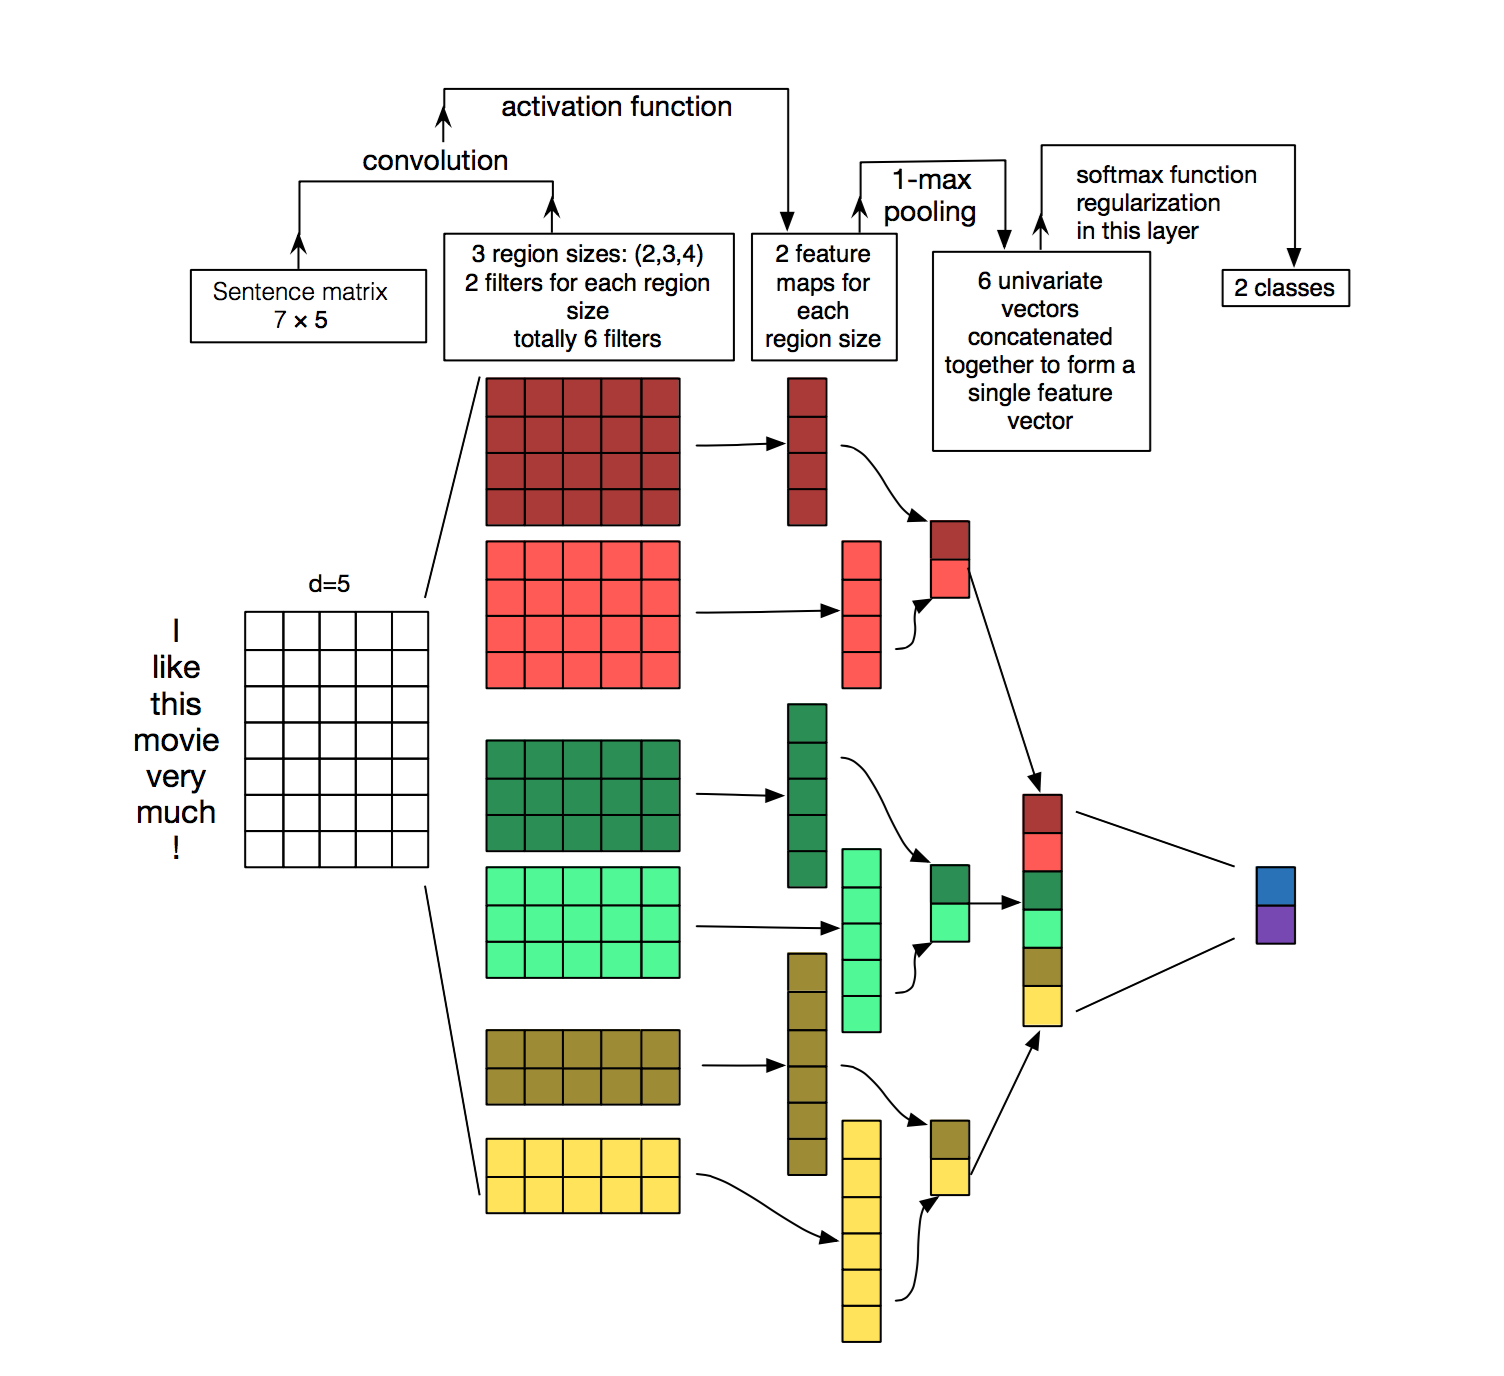
\includegraphics[width=1.0\textwidth]{cnn_nlp_architecture.png}
    \captionof{figure}{Kiến trúc CNN cho phân loại văn bản. Các bộ lọc có kích thước khác nhau (2, 3, 4 từ) trượt dọc theo câu để trích xuất các đặc trưng N-gram. Kết quả sau đó được gộp lại (max-pooling) và đưa vào một lớp FNN để phân loại.}
    \label{fig:cnn_nlp_architecture}
\end{center}

\subsection{Kiến trúc và Dòng chảy Dữ liệu}
\label{ssec:cnn_architecture}
Một kiến trúc CNN điển hình cho bài toán phân loại văn bản bao gồm bốn thành phần chính:

\subsubsection{1. Lớp Nhúng (Embedding Layer)}
Đây là bước đầu tiên, biến đổi câu đầu vào từ một chuỗi các chỉ số từ (word indices) thành một ma trận.
\begin{itemize}
    \item \textbf{Đầu vào:} Một câu, ví dụ "NLP rất thú vị và mạnh mẽ".
    \item \textbf{Đầu ra:} Một ma trận có kích thước (\texttt{số\_từ}, chiều\_embedding). Ví dụ, (6, 300).
\end{itemize}

\subsubsection{2. Lớp Tích chập (Convolutional Layer)}
Đây là trái tim của mô hình, nơi các đặc trưng được trích xuất.
\paragraph{Trực giác cốt lõi}
Trong NLP, một bộ lọc 1D có thể được xem như một \textbf{bộ phát hiện N-gram (N-gram detector)}. Một bộ lọc có chiều cao là 2 từ (`height=2`) sẽ học cách phát hiện các mẫu bigram quan trọng. Một bộ lọc có chiều cao là 3 (`height=3`) sẽ học cách phát hiện các mẫu trigram quan trọng.

\paragraph{Hoạt động}
\begin{itemize}
    \item \textbf{Bộ lọc (Filter):} Một bộ lọc là một ma trận trọng số nhỏ, có kích thước (\texttt{kích\_thước\_N-gram}, \texttt{chiều\_embedding}). Ví dụ, một bộ lọc trigram sẽ có kích thước (3, 300).
    \item \textbf{Phép tích chập:} Bộ lọc này sẽ \textbf{trượt (slides)} dọc theo ma trận embedding của câu, từ trên xuống dưới, mỗi lần một bước. Tại mỗi vị trí, nó thực hiện một phép tích vô hướng (dot product) giữa các trọng số của nó và vùng ma trận embedding mà nó bao phủ. Kết quả của mỗi phép tích là một con số duy nhất.
    \item \textbf{Bản đồ Đặc trưng (Feature Map):} Sau khi trượt hết câu, bộ lọc sẽ tạo ra một chuỗi các con số, gọi là một \textbf{bản đồ đặc trưng}. Chuỗi này biểu diễn sự hiện diện của mẫu N-gram mà bộ lọc đó được "chuyên môn hóa" để phát hiện tại các vị trí khác nhau trong câu.
\end{itemize}

Thông thường, chúng ta không chỉ dùng một bộ lọc. Chúng ta sử dụng \textbf{nhiều bộ lọc} cho mỗi kích thước N-gram (ví dụ: 100 bộ lọc cho bigram, 100 bộ lọc cho trigram, 100 bộ lọc cho 4-gram). Mỗi bộ lọc sẽ tự học để phát hiện một loại mẫu N-gram khác nhau (ví dụ: một bộ lọc bigram có thể chuyên phát hiện các mẫu "rất + [tính từ tích cực]", một bộ lọc khác chuyên phát hiện "không + [động từ]").
\begin{tcolorbox}[
    title=Ghi chú sâu về Lớp Nhúng và Tích chập,
    colback=green!5!white, colframe=green!50!black, fonttitle=\bfseries
]
\textbf{1. Fine-tuning Embeddings và Multiple Channels} \\
Một quyết định quan trọng là có nên cập nhật các vector embedding trong quá trình huấn luyện hay không.
\begin{itemize}
    \item \textbf{Static (Tĩnh):} Sử dụng embedding đã được huấn luyện trước (pre-trained) và giữ cố định. Đây là lựa chọn tốt khi tập dữ liệu cho tác vụ hiện tại nhỏ, để tránh overfitting.
    \item \textbf{Non-static (Động):} Cho phép mô hình "tinh chỉnh" (fine-tune) các embedding. Điều này giúp các vector từ học được những sắc thái ngữ nghĩa đặc thù cho tác vụ đang giải quyết. Ví dụ, trong bài toán phân tích cảm xúc, embedding của từ "tuyệt vời" có thể được đẩy ra xa hơn embedding của từ "tốt".
    \item \textbf{Multiple Channels:} Một kỹ thuật mạnh mẽ là sử dụng nhiều "kênh" đầu vào. Ví dụ, một kênh là embedding tĩnh, kênh kia là embedding động. Các bộ lọc tích chập sẽ học cách trích xuất đặc trưng từ cả hai kênh này. Ý tưởng này tương tự như các kênh màu (RGB) trong ảnh, cho phép mô hình tiếp cận dữ liệu từ nhiều "góc nhìn" khác nhau.
\end{itemize}

\textbf{2. Tại sao chiều rộng của bộ lọc bằng chiều embedding?} \\
Bộ lọc trong CNN cho NLP được thiết kế để có chiều rộng bằng với chiều của embedding (ví dụ, $3 \times 300$ cho một trigram detector). Điều này là có chủ ý. Mục đích là để bộ lọc xem xét \textbf{toàn bộ thông tin ngữ nghĩa} của một từ tại một thời điểm, chứ không phải chỉ một vài chiều riêng lẻ. Phép tích chập sau đó sẽ kết hợp thông tin từ tất cả các chiều của các từ trong cửa sổ N-gram để tạo ra một giá trị đặc trưng duy nhất. Nó không trượt theo chiều embedding, mà chỉ trượt theo chiều dài của câu.
\end{tcolorbox}
\subsubsection{3. Lớp Gộp (Pooling Layer)}
Sau lớp tích chập, chúng ta có rất nhiều bản đồ đặc trưng, mỗi cái là một vector dài. Lớp gộp có nhiệm vụ giảm chiều dữ liệu và tóm tắt thông tin quan trọng nhất từ mỗi bản đồ đặc trưng.

\paragraph{Trực giác cốt lõi}
Lớp gộp trả lời câu hỏi: "Đối với mẫu N-gram mà bộ lọc này phát hiện, liệu nó có xuất hiện một cách \textbf{nổi bật} ở đâu đó trong câu không?". Chúng ta không quan tâm nó xuất hiện ở đâu, chỉ cần biết nó có xuất hiện hay không.

\paragraph{Hoạt động: Max-over-time Pooling}
Kỹ thuật gộp phổ biến nhất trong NLP là \textbf{Max-over-time Pooling} (gọi tắt là Max-Pooling).
\begin{itemize}
    \item Đối với mỗi bản đồ đặc trưng (vector), nó chỉ đơn giản là lấy ra \textbf{giá trị lớn nhất (maximum value)}.
    \item Giá trị lớn nhất này đại diện cho tín hiệu mạnh nhất của mẫu N-gram tương ứng trong toàn bộ câu.
    \item Sau bước này, mỗi bộ lọc chỉ đóng góp một con số duy nhất. Nếu chúng ta có 100 bộ lọc bigram, 100 bộ lọc trigram, và 100 bộ lọc 4-gram, kết quả của lớp gộp sẽ là một vector 300 chiều.
\end{itemize}
\paragraph{Tại sao Max-Pooling lại hiệu quả?}
Trực giác đằng sau sự thành công của Max-pooling trong phân loại văn bản là nó hoạt động như một cơ chế phát hiện đặc trưng. Mỗi bản đồ đặc trưng là đầu ra của một "bộ phát hiện N-gram" cụ thể. Bằng cách lấy giá trị lớn nhất, chúng ta đang trả lời câu hỏi: "Tín hiệu của N-gram quan trọng này có xuất hiện mạnh mẽ nhất ở đâu đó trong câu không?".
\begin{itemize}
    \item Nó tạo ra sự \textbf{bất biến về vị trí (positional invariance)}. Mô hình không quan tâm cụm từ "rất tệ" xuất hiện ở đầu hay cuối câu, miễn là nó xuất hiện và tạo ra một tín hiệu mạnh.
    \item Nó tập trung vào các tín hiệu \textbf{nổi bật nhất}, bỏ qua các tín hiệu nhiễu hoặc yếu hơn. Trong phân loại cảm xúc, chỉ cần một cụm từ tiêu cực mạnh là đủ để quyết định nhãn của cả câu.
    \item \textbf{Average-pooling}, ngược lại, sẽ làm "trung hòa" tín hiệu. Nếu một câu có một cụm từ rất tích cực và nhiều cụm từ trung tính, giá trị trung bình sẽ bị kéo xuống, làm mất đi đặc trưng quan trọng nhất.
\end{itemize}
\subsubsection{4. Lớp Kết nối Đầy đủ, Phân loại, và Huấn luyện}
Vector đặc trưng cuối cùng (ví dụ, 300 chiều) từ lớp gộp giờ đây đã nắm bắt được những thông tin N-gram quan trọng nhất của câu. Vector này được đưa vào một mạng nơ-ron truyền thẳng (FNN) thông thường, thường có một hoặc hai lớp ẩn và một lớp softmax ở cuối để đưa ra dự đoán phân loại cuối cùng.

Quá trình huấn luyện của toàn bộ mạng được thực hiện end-to-end. Hàm mất mát (thường là Cross-Entropy) được tính toán dựa trên dự đoán của lớp softmax và nhãn thật. Sau đó, gradient của lỗi sẽ được lan truyền ngược (\textbf{backpropagation}) qua toàn bộ mạng, từ lớp FNN, qua lớp gộp, đến lớp tích chập để cập nhật trọng số của các bộ lọc, và có thể cập nhật cả lớp embedding (nếu ở chế độ non-static).

\subsection{Ưu và Nhược điểm của CNN cho NLP}
\begin{tcolorbox}[
    title=Đánh giá CNN cho NLP,
    colback=blue!5!white, colframe=blue!50!black, fonttitle=\bfseries
]
\textbf{Ưu điểm:}
\begin{itemize}
    \item \textbf{Cực kỳ hiệu quả tính toán:} Phép tích chập có thể được song song hóa ở mức độ cao, làm cho CNN nhanh hơn đáng kể so với RNN/LSTM trong quá trình huấn luyện.
    \item \textbf{Trích xuất đặc trưng cục bộ tốt:} CNN rất giỏi trong việc phát hiện các mẫu N-gram quan trọng, bất kể chúng xuất hiện ở đâu trong câu (nhờ vào lớp gộp). Điều này rất hữu ích cho các bài toán mà sự hiện diện của các cụm từ khóa là yếu tố quyết định, như phân tích cảm xúc hay phân loại chủ đề.
    \item \textbf{Kiến trúc đơn giản:} So với LSTM, kiến trúc CNN dễ hiểu và triển khai hơn.
\end{itemize}
\textbf{Nhược điểm:}
\begin{itemize}
    \item \textbf{Không nhạy cảm với trật tự từ tầm xa:} Do kích thước của các bộ lọc bị giới hạn, CNN chỉ có thể nắm bắt các phụ thuộc cục bộ (trong phạm vi N-gram). Nó không thể hiểu các mối quan hệ ngữ pháp phức tạp giữa các từ ở hai đầu của một câu dài như cách LSTM có thể làm.
    \item \textbf{Không phù hợp cho các tác vụ sinh ngôn ngữ (NLG):} Bản chất của CNN là trích xuất đặc trưng để phân loại, không phải để sinh ra một chuỗi mới.
\end{itemize}
\end{tcolorbox}
\subsection{Các Kiến trúc CNN Nâng cao và Ứng dụng}
Kiến trúc CNN cơ bản đã rất mạnh mẽ, nhưng có nhiều biến thể nâng cao đã được phát triển để giải quyết các vấn đề phức tạp hơn:

\paragraph{Mạng CNN Đa lớp (Stacked/Multi-layer CNNs)}
Giống như trong xử lý ảnh, chúng ta có thể xếp chồng nhiều lớp tích chập và gộp lên nhau.
\begin{itemize}
    \item \textbf{Ý tưởng:} Lớp CNN đầu tiên học các đặc trưng N-gram từ văn bản thô. Lớp CNN thứ hai sẽ thực hiện tích chập trên đầu ra của lớp đầu tiên, do đó nó học được các \textbf{tổ hợp của các N-gram} (ví dụ, một quy luật về sự xuất hiện của một bigram tích cực sau một trigram tiêu cực).
    \item \textbf{Ứng dụng:} Cho phép mô hình học các đặc trưng ngữ nghĩa ở mức độ trừu tượng cao hơn, hữu ích cho các bài toán phân loại phức tạp.
\end{itemize}

\paragraph{Mạng CNN ở Cấp độ Ký tự (Character-level CNNs)}
Thay vì áp dụng tích chập trên các từ, chúng ta có thể áp dụng nó trên các ký tự.
\begin{itemize}
    \item \textbf{Cơ chế:} Một từ được biểu diễn như một ma trận (\texttt{số\_ký\_tự}, \texttt{chiều\_embedding\_ký\_tự}). Một CNN sẽ trượt qua ma trận này để tạo ra một vector biểu diễn cho từ đó. Vector này sau đó có thể được đưa vào một RNN/LSTM ở cấp độ từ.
    \item \textbf{Ưu điểm:}
        \begin{enumerate}
            \item \textbf{Xử lý từ OOV:} Mô hình có thể tạo ra biểu diễn cho bất kỳ từ nào, kể cả từ chưa từng thấy, dựa trên các ký tự cấu thành nó.
            \item \textbf{Hiểu hình thái học:} Nó có thể nhận ra các tiền tố, hậu tố, và gốc từ (ví dụ, "running", "ran", "runner" đều chứa "run"), giúp mô hình hiểu được mối quan hệ giữa các từ cùng họ.
        \end{enumerate}
\end{itemize}
Những kiến trúc nâng cao này cho thấy sự linh hoạt và sức mạnh của phép tích chập như một công cụ trích xuất đặc trưng hiệu quả trong NLP.
\subsection{So sánh CNN và RNN cho NLP}
CNN và RNN tiếp cận bài toán xử lý văn bản từ hai góc độ hoàn toàn khác nhau:
\begin{itemize}
    \item \textbf{RNN/LSTM} xem văn bản như một chuỗi tuần tự, xử lý từng bước một và xây dựng một "trí nhớ" về quá khứ. Nó rất mạnh trong việc mô hình hóa các phụ thuộc tầm xa và các tác vụ yêu cầu hiểu sâu về cấu trúc câu.
    \item \textbf{CNN} xem văn bản như một "túi các N-gram", sử dụng các bộ lọc để tìm kiếm các mẫu cục bộ quan trọng. Nó rất mạnh trong việc trích xuất các đặc trưng phân loại hiệu quả và nhanh chóng.
\end{itemize}
Trong thực tế, người ta cũng thường kết hợp cả hai kiến trúc này (ví dụ, sử dụng CNN để trích xuất đặc trưng từ ký tự, sau đó đưa vào một LSTM để xử lý ở cấp độ từ) để tận dụng thế mạnh của cả hai.